% Camera-ready exploratory agent robustness analysis.
% These gateway configurations must not be described as human participants or
% direct evaluations of consumer chat products.
\subsection{Multi-Model Agent Robustness Analysis}
\label{sec:multi-model-agent-analysis}

We further examine whether OpenCoder's uncertainty presentation changes the
behavior of automated code reviewers. Twelve gateway-mediated model
configurations---GPT, Claude, Gemini, DeepSeek, Qwen, Kimi, Grok, Llama, GLM,
MiniMax, Doubao, and ERNIE---each reviewed 12 frozen ExecRepoBench tasks under
a counterbalanced design. The study therefore comprised 144 independent
episodes, with 48 episodes assigned to each of generic review, aggregate
uncertainty display, and source-specific targeted guidance. Models received no
test outcomes, hidden reference code, tools, or conversational history. Every
returned target function was assessed with the same private executable tests.

Figure~\ref{fig:agent-review-summary} summarizes the aggregate outcomes. Generic
review achieved 38.6\% correctness among executable outputs and 35.4\%
end-to-end success over all planned episodes. Aggregate uncertainty display
increased these descriptive rates to 46.7\% and 43.8\%, respectively. Its
end-to-end difference from generic review was +8.3 percentage points, although
the model-clustered 95\% bootstrap interval included zero
($[-2.1,+18.8]$). Source-specific targeted guidance achieved 35.6\%
correctness among executable outputs and 33.3\% end-to-end success, a
$-2.1$-point difference from generic review ($95\%$ CI
$[-12.5,+8.3]$). Thus, this campaign does not support a claim that targeted
guidance is superior across model families.

Figure~\ref{fig:gateway-campaign-coverage} reports the resolved gateway
configurations and campaign audit. The final artifact contains 144 unique
records, including 134 executable outputs and 10 model-side missing outputs,
with no evaluator infrastructure errors or served-model mismatches. The
gateway reported 599,210 tokens across the campaign. Missing outputs were
excluded from executable-output correctness and retained in the denominator of
the end-to-end sensitivity analysis.

\noindent\textbf{Finding.}
The aggregate uncertainty display yielded the strongest descriptive agent
outcomes, but the uncertainty interval does not establish a reliable positive
effect. Source-specific guidance did not improve aggregate performance. We
therefore treat this experiment as a robustness analysis of uncertainty
presentation across gateway-mediated model configurations, not as evidence of
human usability or direct evaluation of consumer chat products.

\begin{figure*}[t]
    \centering
    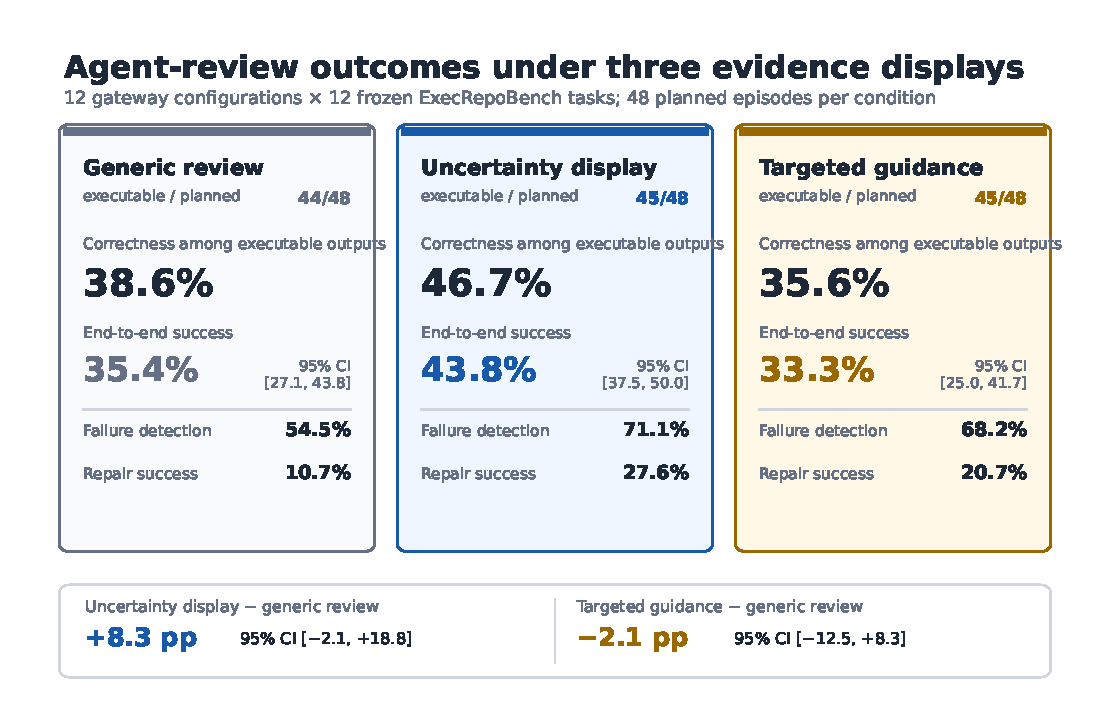
\includegraphics[width=\textwidth]{figures/fig_agent_review_boxed.pdf}
    \caption{Executable review outcomes across three evidence-display
    conditions. Correctness uses only executable model outputs; end-to-end
    success retains all 48 planned episodes per condition. Intervals are
    model-clustered 95\% bootstrap intervals over 10,000 resamples.}
    \label{fig:agent-review-summary}
\end{figure*}

\begin{figure*}[t]
    \centering
    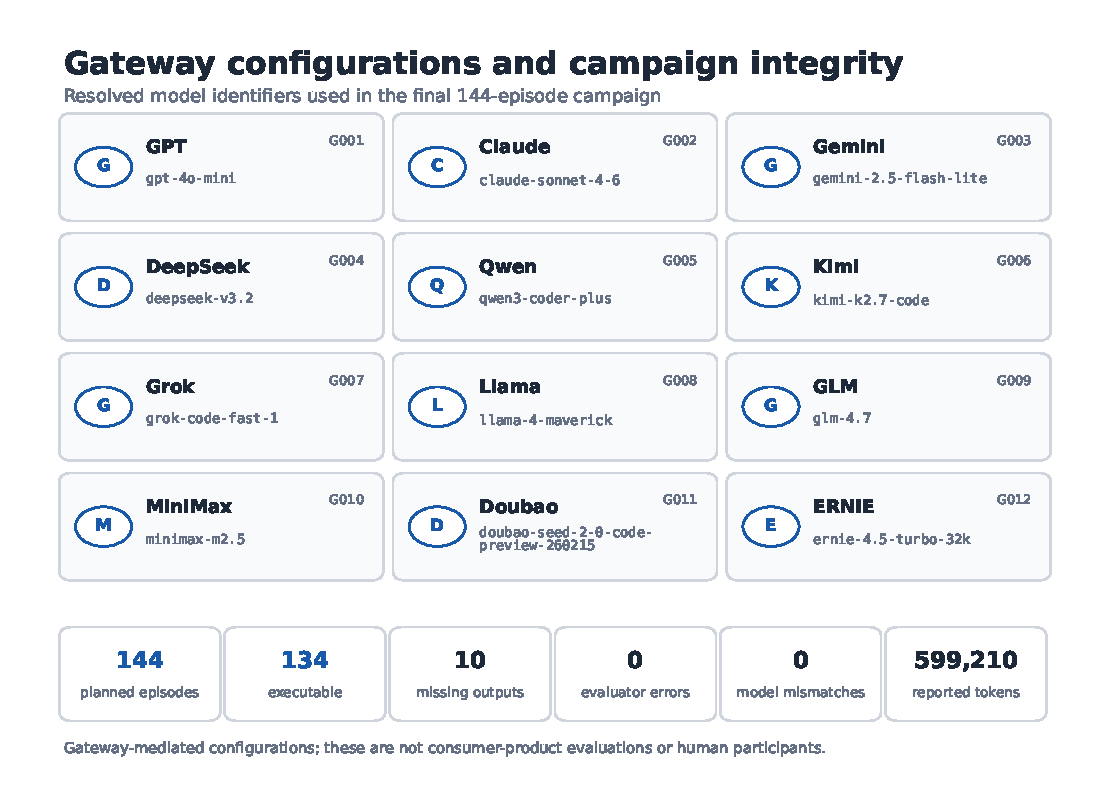
\includegraphics[width=\textwidth]{figures/fig_gateway_campaign_coverage.pdf}
    \caption{Resolved gateway configurations and integrity summary for the
    exploratory multi-model campaign. Model names denote API configurations,
    not consumer chat products.}
    \label{fig:gateway-campaign-coverage}
\end{figure*}
